\documentclass[ignorenonframetext]{beamer}

%\documentclass[handout,ignorenonframetext]{beamer}

% Standardni paketi:
\usepackage[slovene]{babel}
\usepackage[utf8]{inputenc}
\usepackage[T1]{fontenc}
\usepackage{lmodern}

% Paketi, s katerimi določimo željene pisave:
\usepackage{mathptmx}
\usepackage{helvet} % splošen font pisave
\usepackage{courier} %font pisave v okolju verbatim

% Kot v article lahko definiramo nova okolja:
\newtheorem{definicija}{Definicija}
\newtheorem{izrek}{Izrek}
\newtheorem{zgled}{Zgled}

\mode<article>{
\setlength{\parindent}{0cm}
\usepackage{amsfonts}
\let\frametitle\subsection %%naslovi slidov postanejo naslovi podrazdelkov v article
}

\mode<beamer>{
\usetheme{Rochester}}

\mode<handout>{
\usetheme{AnnArbor}

\useoutertheme{infolines} %določi glavo in nogo
\setbeamercovered{transparent} %neodkriti tekst je rahlo viden
\setbeamercolor{background canvas}{bg=black!5}
\usepackage{pgfpages} %2 na 1 stran
\pgfpagesuselayout{2 on 1}[a4paper, border shrink=5mm]
}

\usepackage{tikz}
\usetikzlibrary{calc}
\usetikzlibrary{arrows,decorations.markings}

\tikzset{
    right angle quadrant/.code={
        \pgfmathsetmacro\quadranta{{1,1,-1,-1}[#1-1]}     % Arrays for selecting quadrant
        \pgfmathsetmacro\quadrantb{{1,-1,-1,1}[#1-1]}},
    right angle quadrant=1, % Make sure it is set, even if not called explicitly
    right angle length/.code={\def\rightanglelength{#1}},   % Length of symbol
    right angle length=2ex, % Make sure it is set...
    right angle symbol/.style n args={3}{
        insert path={
            let \p0 = ($(#1)!(#3)!(#2)$) in     % Intersection
                let \p1 = ($(\p0)!\quadranta*\rightanglelength!(#3)$), % Point on base line
                \p2 = ($(\p0)!\quadrantb*\rightanglelength!(#2)$) in % Point on perpendicular line
                let \p3 = ($(\p1)+(\p2)-(\p0)$) in  % Corner point of symbol
            (\p1) -- (\p3) -- (\p2)
        }
    }
}

\title{Spojena kubična Bezierjeva krpa}
\author{Matija Šteblaj, Nejc Ševerkar}
\date{14. 1. 2021}

\begin{document}

\begin{frame}
\titlepage
\end{frame}

\begin{frame}
\frametitle{Motivacija}
Želimo poiskati preprosto $C^1$-ploskev, ki v danih točkah (iz $\mathbb{R}^2$) interpolira predpisane vrednosti in parcialne odvode (npr. od neke funkcije).\vspace{10px}

Ideja: naredimo triangulacijo na točkah in definiramo lokalno shemo na vsakem trikotniku posebej, kjer poskrbimo za ustrezna ujemanja na presekih (stranicah) trikotnikov. Tu si bomo pomagali z Bézierjevimi krpami stopnje 3.
\end{frame}


\begin{frame}
\frametitle{Klasična  Bézierjeva krpa stopnje 3}
Spomnimo se, da je parametrizacija  Bézierjeve krpe stopnje 3 na nekem trikotniku podana s točkami $b_{ijk}, i+j+k=3$ kot:
\[
\begin{split}
	P(u,v,w) =& \sum_{i+j+k=3} b_{ijk} B_{ijk}^3(u,v,w) \\
		=& u^3 \text{ }b_{300} + 3u^2 v \text{ }b_{210} + 3u^2 w \text{ }b_{201} + 3u v^2 \text{ }b_{120} \\
		&+ 3uw^2 \text{ }b_{102} + v^3 \text{ }b_{030} + 3v^2 w \text{ }b_{021} + 3v w^2 \text{ }b_{012} \\
		&+ w^3 \text{ }b_{003} + 6uvw \text{ }b_{111}
\end{split}
\]
in njen odvod v smeri $\textbf{z} = (z_u,z_v,z_w)$ enak:
$$\frac{\partial{P}}{\partial{\textbf{z}}} = \frac{\partial{P}}{\partial{u}} z_u+ \frac{\partial{P}}{\partial{v}} z_v+ \frac{\partial{P}}{\partial{w}} z_w = <\text{grad}(P), \textbf{z}>\text{,}$$
kjer $u,v,w$ predstavljajo baricentrične koordinate v danem trikotniku.
\end{frame}

\begin{frame}
\frametitle{Shema}
Recimo, da triangulacijo že imamo, in vzemimo nek trikotnik v domeni:
	\begin{figure}
		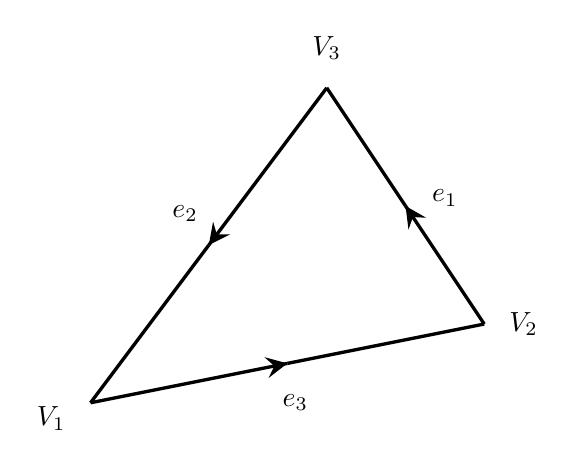
\begin{tikzpicture}%[scale=0.8]
			\node (sidro) at (0,0) {};
			
			\node (V1) at ($(sidro)+(-3,-1)$) {};
			\node (p1) at ($(V1) + (-0.5, -0.2)$){$V_1$};
			\node (V15) at ($(V1) + (2.5, 0.5)$){};
			\node (V2) at ($(sidro)+(2,0)$) {};
			\node (p2) at ($(V2) + (0.5, 0)$){$V_2$};
			\node (V25) at ($(V2) + (-1, 1.5)$){};
			\node (V3) at ($(sidro)+(0,3)$) {};
			\node (p3) at ($(V3) + (0, 0.5)$){$V_3$};
			\node (V35) at ($(V3) + (-1.5, -2)$){};
			%vektor e_1 = (5,1), e_2 = (-2,3), e_3 = (-3,-4)

			\node (e1) at ($(V25) + (0.5,0.1)$){$e_1$};
			\node (e2) at ($(V35) + (-0.3,0.4)$){$e_2$};
			\node (e3) at ($(V15) + (0.1,-0.5)$){$e_3$};


			\draw[very thick, black,decoration={markings,mark=at position 1 with {\arrow[scale=1.5,>=stealth]{>}}},postaction={decorate}] (V1.center) -- (V15.center);
			\draw[very thick, black] (V15.center) -- (V2.center);
			\draw[very thick, black,decoration={markings,mark=at position 1 with {\arrow[scale=1.5,>=stealth]{>}}},postaction={decorate}] (V2.center) -- (V25.center);
			\draw[very thick, black] (V25.center) -- (V3.center);
			\draw[very thick, black,decoration={markings,mark=at position 1 with {\arrow[scale=1.5,>=stealth]{>}}},postaction={decorate}] (V3.center) -- (V35.center);
			\draw[very thick, black] (V35.center) -- (V1.center);

		\end{tikzpicture}
	\end{figure}
\end{frame}

\begin{frame}
\frametitle{Shema}
Določiti moramo točke kontrolne mreže $b_{ijk}$ nad tem trikotnikom:
	\begin{figure}
		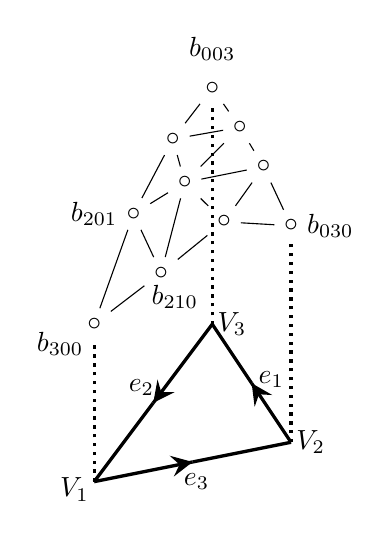
\begin{tikzpicture}[scale=0.5]
			\node (sidro) at (0,0) {};
			
			\node (V1) at ($(sidro)+(-3,-1)$) {};
			\node (p1) at ($(V1) + (-0.5, -0.2)$){$V_1$};
			\node (V15) at ($(V1) + (2.5, 0.5)$){};
			\node (V2) at ($(sidro)+(2,0)$) {};
			\node (p2) at ($(V2) + (0.5, 0)$){$V_2$};
			\node (V25) at ($(V2) + (-1, 1.5)$){};
			\node (V3) at ($(sidro)+(0,3)$) {};
			\node (p3) at ($(V3) + (0:0.5)$){$V_3$};
			\node (V35) at ($(V3) + (-1.5, -2)$){};
			%vektor e_3 = (5,1), e_1 = (-2,3), e_2 = (-3,-4)

			\node (b300) at ($(V1) + (0,4)$){$\circ$};
			\node (300) at ($(b300) + (210:1)$){$b_{300}$};
			\node (b003) at ($(V3) + (0,6)$){$\circ$};
			\node (003) at ($(b003) + (90:1)$){$b_{003}$};
			\node (b030) at ($(V2) + (0,5.5)$){$\circ$};
			\node (030) at ($(b030) + (0:1)$){$b_{030}$};

			\node(b201) at ($(V1) + (1, 1.3) + (0,5.5)$){$\circ$};
			\node(201) at ($(b201) + (180:1)$){$b_{201}$};
			\node(b102) at ($(V1) + (2, 2.7) + (0,6)$){$\circ$};


			\node(b210) at ($(V1) + (1.7, 0.3) + (0,5)$){$\circ$};
			\node(210) at ($(b210) + (300:0.7)$){$b_{210}$};
			\node(b120) at ($(V1) + (3.3, 0.6) + (0,6)$){$\circ$};

			\node(b021) at ($(V2) + (-0.7, 1) + (0,6)$){$\circ$};
			\node(b012) at ($(V2) + (-1.3, 1) + (0,7)$){$\circ$};

			\node(b111) at ($(V1) + (3.3,0.6) + (-1,1.5) +(0,5.5)$){$\circ$};


			\node (e1) at ($(V25) + (0.5,0.1)$){$e_1$};
			\node (e2) at ($(V35) + (-0.3,0.4)$){$e_2$};
			\node (e3) at ($(V15) + (0.1,-0.5)$){$e_3$};


			\draw[very thick, black,decoration={markings,mark=at position 1 with {\arrow[scale=1.5,>=stealth]{>}}},postaction={decorate}] (V1.center) -- (V15.center);
			\draw[very thick, black] (V15.center) -- (V2.center);
			\draw[very thick, black,decoration={markings,mark=at position 1 with {\arrow[scale=1.5,>=stealth]{>}}},postaction={decorate}] (V2.center) -- (V25.center);
			\draw[very thick, black] (V25.center) -- (V3.center);
			\draw[very thick, black,decoration={markings,mark=at position 1 with {\arrow[scale=1.5,>=stealth]{>}}},postaction={decorate}] (V3.center) -- (V35.center);
			\draw[very thick, black] (V35.center) -- (V1.center);

			\draw[very thick, black, dotted] (V1.center) -- (b300);
			\draw[very thick, black, dotted] (V2.center) -- (b030);
			\draw[very thick, black, dotted] (V3.center) -- (b003);

			\draw[black] (b300) -- (b210);
			\draw[black] (b300) -- (b201);

			\draw[black] (b210) -- (b120);
			\draw[black] (b210) -- (b111);
			\draw[black] (b210) -- (b201);

			\draw[black] (b201) -- (b111);
			\draw[black] (b201) -- (b102);

			\draw[black] (b102) -- (b111);
			\draw[black] (b102) -- (b003);
			\draw[black] (b102) -- (b012);

			\draw[black] (b003) -- (b012);

			\draw[black] (b012) -- (b021);
			\draw[black] (b012) -- (b111);

			\draw[black] (b120) -- (b111);
			\draw[black] (b120) -- (b021);

			\draw[black] (b021) -- (b111);

			\draw[black] (b030) -- (b120);
			\draw[black] (b030) -- (b021);

		\end{tikzpicture}
	\end{figure}
\end{frame}

\begin{frame}
\frametitle{Shema}
Predpisane imamo vrednosti $F(V_i)$ in parcialne odvode $F_x(V_i), F_y(V_i)$ za $V_i = (x_i, y_i)$ $i=1,2,3$. Od tod lahko dobimo smerne odvode v smeri stranic kot:
$$F_{e_i} = \frac{\partial{F}}{\partial{e_i}}  = (x_{i-1}- x_{i+1}) F_x + (y_{i-1}-y_{i+1}) F_y = <e_i,\text{grad}(F)>$$

S pomočjo tega lahko definiramo točke ``okoli'' enega oglišča trikotnika:
\[
\begin{split}
	b_{300} =& F(V_1) \\
	b_{210} =& F(V_1) + \frac{F_{e_3}}{3} \\
	b_{201} =& F(V_1) - \frac{F_{e_2}}{3}
\end{split}
\]

\end{frame}

\begin{frame}
\frametitle{Shema}
$$b_{300} = F(V_1), b_{210} = F(V_1) + \frac{F_{e_3}}{3}, b_{201} = F(V_1) - \frac{F_{e_2}}{3}$$
	\begin{figure}
		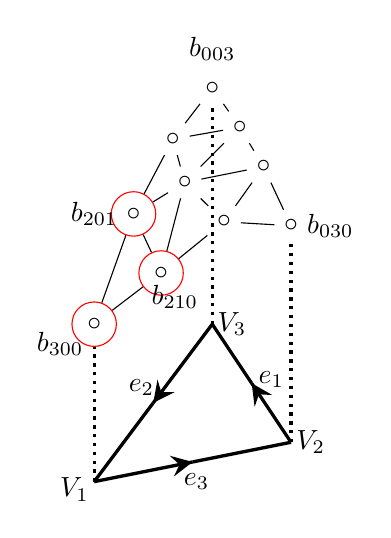
\begin{tikzpicture}[scale=0.5, roundnode/.style={circle, draw=red}]
			\node (sidro) at (0,0) {};
			
			\node (V1) at ($(sidro)+(-3,-1)$) {};
			\node (p1) at ($(V1) + (-0.5, -0.2)$){$V_1$};
			\node (V15) at ($(V1) + (2.5, 0.5)$){};
			\node (V2) at ($(sidro)+(2,0)$) {};
			\node (p2) at ($(V2) + (0.5, 0)$){$V_2$};
			\node (V25) at ($(V2) + (-1, 1.5)$){};
			\node (V3) at ($(sidro)+(0,3)$) {};
			\node (p3) at ($(V3) + (0:0.5)$){$V_3$};
			\node (V35) at ($(V3) + (-1.5, -2)$){};
			%vektor e_3 = (5,1), e_1 = (-2,3), e_2 = (-3,-4)

			\node[roundnode] (b300) at ($(V1) + (0,4)$){$\circ$};
			\node (300) at ($(b300) + (210:1)$){$b_{300}$};
			\node (b003) at ($(V3) + (0,6)$){$\circ$};
			\node (003) at ($(b003) + (90:1)$){$b_{003}$};
			\node (b030) at ($(V2) + (0,5.5)$){$\circ$};
			\node (030) at ($(b030) + (0:1)$){$b_{030}$};

			\node[roundnode] (b201) at ($(V1) + (1, 1.3) + (0,5.5)$){$\circ$};
			\node(201) at ($(b201) + (180:1)$){$b_{201}$};
			\node(b102) at ($(V1) + (2, 2.7) + (0,6)$){$\circ$};


			\node[roundnode](b210) at ($(V1) + (1.7, 0.3) + (0,5)$){$\circ$};
			\node(210) at ($(b210) + (300:0.7)$){$b_{210}$};
			\node(b120) at ($(V1) + (3.3, 0.6) + (0,6)$){$\circ$};

			\node(b021) at ($(V2) + (-0.7, 1) + (0,6)$){$\circ$};
			\node(b012) at ($(V2) + (-1.3, 1) + (0,7)$){$\circ$};

			\node(b111) at ($(V1) + (3.3,0.6) + (-1,1.5) +(0,5.5)$){$\circ$};


			\node (e1) at ($(V25) + (0.5,0.1)$){$e_1$};
			\node (e2) at ($(V35) + (-0.3,0.4)$){$e_2$};
			\node (e3) at ($(V15) + (0.1,-0.5)$){$e_3$};


			\draw[very thick, black,decoration={markings,mark=at position 1 with {\arrow[scale=1.5,>=stealth]{>}}},postaction={decorate}] (V1.center) -- (V15.center);
			\draw[very thick, black] (V15.center) -- (V2.center);
			\draw[very thick, black,decoration={markings,mark=at position 1 with {\arrow[scale=1.5,>=stealth]{>}}},postaction={decorate}] (V2.center) -- (V25.center);
			\draw[very thick, black] (V25.center) -- (V3.center);
			\draw[very thick, black,decoration={markings,mark=at position 1 with {\arrow[scale=1.5,>=stealth]{>}}},postaction={decorate}] (V3.center) -- (V35.center);
			\draw[very thick, black] (V35.center) -- (V1.center);

			\draw[very thick, black, dotted] (V1.center) -- (b300);
			\draw[very thick, black, dotted] (V2.center) -- (b030);
			\draw[very thick, black, dotted] (V3.center) -- (b003);

			\draw[black] (b300) -- (b210);
			\draw[black] (b300) -- (b201);

			\draw[black] (b210) -- (b120);
			\draw[black] (b210) -- (b111);
			\draw[black] (b210) -- (b201);

			\draw[black] (b201) -- (b111);
			\draw[black] (b201) -- (b102);

			\draw[black] (b102) -- (b111);
			\draw[black] (b102) -- (b003);
			\draw[black] (b102) -- (b012);

			\draw[black] (b003) -- (b012);

			\draw[black] (b012) -- (b021);
			\draw[black] (b012) -- (b111);

			\draw[black] (b120) -- (b111);
			\draw[black] (b120) -- (b021);

			\draw[black] (b021) -- (b111);

			\draw[black] (b030) -- (b120);
			\draw[black] (b030) -- (b021);

		\end{tikzpicture}
	\end{figure}

\end{frame}

\begin{frame}
\frametitle{Shema}
Na analogen način določimo še ostale ``robne'' točke:
	\begin{figure}
		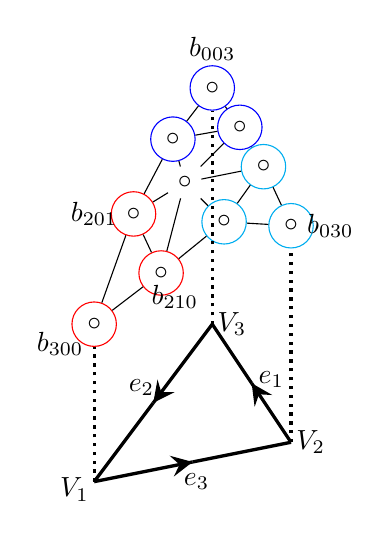
\begin{tikzpicture}[scale=0.5, roundnode/.style={circle, draw=red}, roundnode2/.style={circle, draw=blue}, roundnode3/.style={circle, draw=cyan}]
			\node (sidro) at (0,0) {};
			
			\node (V1) at ($(sidro)+(-3,-1)$) {};
			\node (p1) at ($(V1) + (-0.5, -0.2)$){$V_1$};
			\node (V15) at ($(V1) + (2.5, 0.5)$){};
			\node (V2) at ($(sidro)+(2,0)$) {};
			\node (p2) at ($(V2) + (0.5, 0)$){$V_2$};
			\node (V25) at ($(V2) + (-1, 1.5)$){};
			\node (V3) at ($(sidro)+(0,3)$) {};
			\node (p3) at ($(V3) + (0:0.5)$){$V_3$};
			\node (V35) at ($(V3) + (-1.5, -2)$){};
			%vektor e_3 = (5,1), e_1 = (-2,3), e_2 = (-3,-4)

			\node[roundnode] (b300) at ($(V1) + (0,4)$){$\circ$};
			\node (300) at ($(b300) + (210:1)$){$b_{300}$};
			\node[roundnode2] (b003) at ($(V3) + (0,6)$){$\circ$};
			\node (003) at ($(b003) + (90:1)$){$b_{003}$};
			\node[roundnode3] (b030) at ($(V2) + (0,5.5)$){$\circ$};
			\node (030) at ($(b030) + (0:1)$){$b_{030}$};

			\node[roundnode] (b201) at ($(V1) + (1, 1.3) + (0,5.5)$){$\circ$};
			\node(201) at ($(b201) + (180:1)$){$b_{201}$};
			\node[roundnode2](b102) at ($(V1) + (2, 2.7) + (0,6)$){$\circ$};


			\node[roundnode](b210) at ($(V1) + (1.7, 0.3) + (0,5)$){$\circ$};
			\node(210) at ($(b210) + (300:0.7)$){$b_{210}$};
			\node[roundnode3](b120) at ($(V1) + (3.3, 0.6) + (0,6)$){$\circ$};

			\node[roundnode3](b021) at ($(V2) + (-0.7, 1) + (0,6)$){$\circ$};
			\node[roundnode2](b012) at ($(V2) + (-1.3, 1) + (0,7)$){$\circ$};

			\node(b111) at ($(V1) + (3.3,0.6) + (-1,1.5) +(0,5.5)$){$\circ$};


			\node (e1) at ($(V25) + (0.5,0.1)$){$e_1$};
			\node (e2) at ($(V35) + (-0.3,0.4)$){$e_2$};
			\node (e3) at ($(V15) + (0.1,-0.5)$){$e_3$};


			\draw[very thick, black,decoration={markings,mark=at position 1 with {\arrow[scale=1.5,>=stealth]{>}}},postaction={decorate}] (V1.center) -- (V15.center);
			\draw[very thick, black] (V15.center) -- (V2.center);
			\draw[very thick, black,decoration={markings,mark=at position 1 with {\arrow[scale=1.5,>=stealth]{>}}},postaction={decorate}] (V2.center) -- (V25.center);
			\draw[very thick, black] (V25.center) -- (V3.center);
			\draw[very thick, black,decoration={markings,mark=at position 1 with {\arrow[scale=1.5,>=stealth]{>}}},postaction={decorate}] (V3.center) -- (V35.center);
			\draw[very thick, black] (V35.center) -- (V1.center);

			\draw[very thick, black, dotted] (V1.center) -- (b300);
			\draw[very thick, black, dotted] (V2.center) -- (b030);
			\draw[very thick, black, dotted] (V3.center) -- (b003);

			\draw[black] (b300) -- (b210);
			\draw[black] (b300) -- (b201);

			\draw[black] (b210) -- (b120);
			\draw[black] (b210) -- (b111);
			\draw[black] (b210) -- (b201);

			\draw[black] (b201) -- (b111);
			\draw[black] (b201) -- (b102);

			\draw[black] (b102) -- (b111);
			\draw[black] (b102) -- (b003);
			\draw[black] (b102) -- (b012);

			\draw[black] (b003) -- (b012);

			\draw[black] (b012) -- (b021);
			\draw[black] (b012) -- (b111);

			\draw[black] (b120) -- (b111);
			\draw[black] (b120) -- (b021);

			\draw[black] (b021) -- (b111);

			\draw[black] (b030) -- (b120);
			\draw[black] (b030) -- (b021);

		\end{tikzpicture}
	\end{figure}

\end{frame}

\begin{frame}
\frametitle{Shema}
Določiti moramo še $b_{111}$. Tu bomo imeli 3 ločene izbire $b_{111}^1$, $b_{111}^2$, $b_{111}^3$, kjer bo $b_{111}^m$ tak, da bo zagotavljal $C^1$-zveznost čez stranico $e_m$.

Poglejmo pogoje za stranico $e_1$, pri ostalih dveh pa potem naredimo simetrično.
\end{frame}

\begin{frame}
\frametitle{Lokalna shema}
Poglejmo si notranjo normalo $n_1$ na stranico $e_1$. Velja:
$$n_1 = -e_3 + \frac{e_3 \cdot e_1}{\lvert e_1 \rvert} \frac{e_1}{\lvert e_1 \rvert}$$
\begin{figure}
		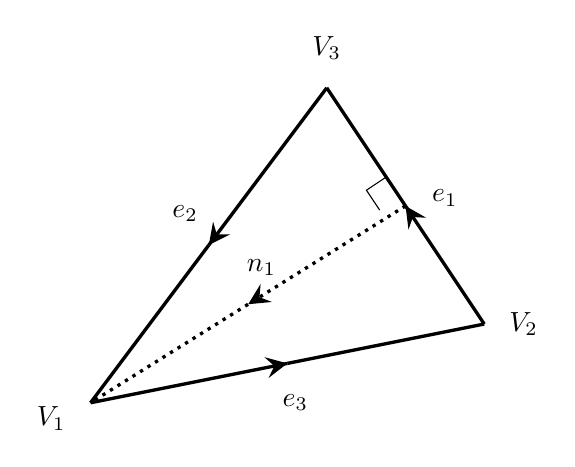
\begin{tikzpicture}
			\node (sidro) at (0,0) {};
			
			\node (V1) at ($(sidro)+(-3,-1)$) {};
			\node (p1) at ($(V1) + (-0.5, -0.2)$){$V_1$};
			\node (V15) at ($(V1) + (2.5, 0.5)$){};
			\node (V2) at ($(sidro)+(2,0)$) {};
			\node (p2) at ($(V2) + (0.5, 0)$){$V_2$};
			\node (V25) at ($(V2) + (-1, 1.5)$){}; %(1,1.5)
			\node (V3) at ($(sidro)+(0,3)$) {};
			\node (p3) at ($(V3) + (0, 0.5)$){$V_3$};
			\node (V35) at ($(V3) + (-1.5, -2)$){};
			%vektor e_3 = (5,1), e_1 = (-2,3), e_2 = (-3,-4), |e_3| / (|e_2| +|e_3|) = ~0.50

			\node (e1) at ($(V25) + (0.5,0.1)$){$e_1$};
			\node (e2) at ($(V35) + (-0.3,0.4)$){$e_2$};
			\node (e3) at ($(V15) + (0.1,-0.5)$){$e_3$};

			\node(H) at ($(V1) + (2, 1.25)$){};
			\node(h) at ($(H) + (70:0.5)$){$n_1$};


			\draw[very thick, black,decoration={markings,mark=at position 1 with {\arrow[scale=1.5,>=stealth]{>}}},postaction={decorate}] (V1.center) -- (V15.center);
			\draw[very thick, black] (V15.center) -- (V2.center);
			\draw[very thick, black,decoration={markings,mark=at position 1 with {\arrow[scale=1.5,>=stealth]{>}}},postaction={decorate}] (V2.center) -- (V25.center);
			\draw[very thick, black] (V25.center) -- (V3.center);
			\draw[very thick, black,decoration={markings,mark=at position 1 with {\arrow[scale=1.5,>=stealth]{>}}},postaction={decorate}] (V3.center) -- (V35.center);
			\draw[very thick, black] (V35.center) -- (V1.center);

			\draw[very thick, black, dotted, decoration={markings,mark=at position 1 with {\arrow[scale=1.5,>=stealth]{>}}},postaction={decorate}] (V25.center)--(H.center);
			\draw[very thick, black, dotted] (H.center)--(V1.center);
			\draw [right angle symbol={V2}{V3}{V1}];

		\end{tikzpicture}
	\end{figure}
\end{frame}

\begin{frame}
\frametitle{Lokalna shema}
Če to enačbo razpišemo v baricentričnih koordinatah:
\[
\begin{split}
	n_1 =& -e_3 + \frac{e_3 \cdot e_1}{\lvert e_1 \rvert} \cdot  \frac{e_1}{\lvert e_1 \rvert}\\
		=& -(-1,1,0) - h_1 (0,-1,1) \\
		=& (1,h_1-1,-h_1) \text{,}
\end{split}
\]
kjer je
$$h_1 = -  \frac{e_3 \cdot e_1}{\lvert e_1 \rvert^2}$$
Če označimo s $P_1$ parametrizacijo B, ki jo dobimo iz prej določenih $b_{ijk}$ in $b_{111}^1$, lahko iz formule poračunamo $\frac{\partial{P_1}}{\partial{n_1}}$.
\end{frame}

\begin{frame}
\frametitle{Lokalna shema}
Odvod $\frac{\partial{P_1}}{\partial{n_1}}$ se na stranici $e_1$ (kjer je $u=0$) poenostavi v:
$$\frac{\partial{P_1}}{\partial{n_1}} = 3I_1 v^2 + 6 I_2 vw + 3I_3 w^2 \text{,}$$
kjer so:
\[
\begin{split}
	I_1 &= b_{120}-b_{030}-h_1(b_{021}-b_{030})\\
	I_2 &= b_{111}^1-b_{021}-h_1(b_{012}-b_{021})\\
	I_3 &= b_{102}-b_{012}-h_1(b_{003}-b_{012})
\end{split}
\]
\end{frame}

\begin{frame}
\frametitle{Lokalna shema}
Z upoštevanjem $w=1-v$, lahko enačbo preoblikujemo v:
$$\frac{\partial{P_1}}{\partial{n_1}} = 3\bigg((I_1-2I_2+I_3) v^2 + 2 (I_2-I_3) v + I_3 \bigg)$$
Zdaj izberemo tak $b_{111}^1$, da bo ta normalni odvod linearen na stranici $e_1$, tj. linearen v parametru $v$. Dobimo torej enačbo:
$$I_1-2I_2+I_3 = 0$$
Od tod lahko izrazimo:
\[
\begin{split}
b_{111}^1 =& \frac{1}{2}\bigg(b_{120}+b_{102}+h_1(2b_{012}-b_{021}-b_{003})\\
		&+(1-h_1)(2b_{021}-b_{030}-b_{012})\bigg)
\end{split}
\]
\end{frame}

\begin{frame}
\frametitle{Lokalna shema}
Zakaj je to dovolj za $C^1$ zveznost čez stranico $e_1$? 

Postopek ponovimo na sosednjem trikotniku in dobimo linearen normalen odvod (v nasprotno smer), kar pomeni da je linearen tudi normalen odvod v smeri 1. trikotnika. Te dva odvoda se ujemata v ogliščih $V_2$, $V_3$ (shema tam interpolira odvode), torej povsod, ker sta linearna.
\begin{figure}
		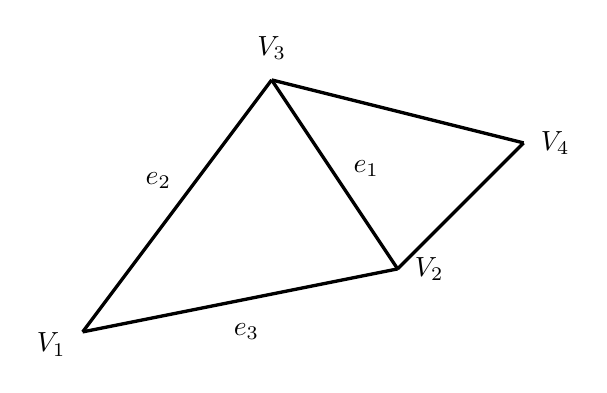
\begin{tikzpicture}[scale=0.8]
			\node (sidro) at (0,0) {};
			
			\node (V1) at ($(sidro)+(-3,-1)$) {};
			\node (p1) at ($(V1) + (-0.5, -0.2)$){$V_1$};
			\node (V15) at ($(V1) + (2.5, 0.5)$){};
			\node (V2) at ($(sidro)+(2,0)$) {};
			\node (p2) at ($(V2) + (0.5, 0)$){$V_2$};
			\node (V25) at ($(V2) + (-1, 1.5)$){};
			\node (V3) at ($(sidro)+(0,3)$) {};
			\node (p3) at ($(V3) + (0, 0.5)$){$V_3$};
			\node (V35) at ($(V3) + (-1.5, -2)$){};

			\node (V4) at ($(sidro) + (4,2)$){};
			\node(p4) at ($(V4) + (0:0.5)$){$V_4$};
			%vektor e_1 = (5,1), e_2 = (-2,3), e_3 = (-3,-4)

			\node (e1) at ($(V25) + (0.5,0.1)$){$e_1$};
			\node (e2) at ($(V35) + (-0.3,0.4)$){$e_2$};
			\node (e3) at ($(V15) + (0.1,-0.5)$){$e_3$};


			\draw[very thick, black] (V1.center) -- (V2.center);
			\draw[very thick, black] (V2.center) -- (V3.center);
			\draw[very thick, black] (V3.center) -- (V1.center);

			\draw[very thick, black] (V3.center) -- (V4.center);
			\draw[very thick, black] (V2.center) -- (V4.center);


		\end{tikzpicture}
	\end{figure}

\end{frame}

\begin{frame}
\frametitle{Celotna shema}
Parametrizacija na celotnem trikotniku bo konveksna kombinacija shem $P_1$, $P_2$, $P_3$:
\[
\begin{split}
	P(u,v,w) =& \frac{v^2 w^2 P_1 + w^2 u^2 P_2 + u^2 v^2 P_3}{v^2 w^2 + v^2 u^2 + u^2 w^2}\\
		=& u^3 \text{ }b_{300} + 3u^2 v \text{ }b_{210} + 3u^2 w \text{ }b_{201} + 3u v^2 \text{ }b_{120} \\
		&+ 3uw^2 \text{ }b_{102} + v^3 \text{ }b_{030} + 3v^2 w \text{ }b_{021} + 3v w^2 \text{ }b_{012} \\
		&+ w^3 \text{ }b_{003} \\
		&+ 6uvw \frac{v^2 w^2 \text{ } b_{111}^1 + w^2 u^2 \text{ } b_{111}^2 + u^2 v^2 \text{ }b_{111}^3}{v^2 w^2 + v^2 u^2 + u^2 w^2}
\end{split}
\]
\end{frame}

\end{document}